% ICML 2026 Paper
% SSL Pretraining with SGD Creates Geometrically Stable Spurious Shortcut Encodings
% Auto-generated by Anonymous Research Pipeline (Phase 6.5.1)
%
% Compile with:
%   pdflatex main.tex
%   bibtex main
%   pdflatex main.tex
%   pdflatex main.tex
%
\documentclass{article}

% ICML 2025 style
\usepackage{icml2025}

% Standard packages
\usepackage{microtype}
\usepackage{graphicx}
\usepackage{booktabs}
\usepackage{hyperref}
\usepackage{amsmath}
\usepackage{amssymb}
\usepackage{algorithm}
\usepackage{algorithmic}
\usepackage{multirow}
\usepackage{makecell}
\usepackage{natbib}

% ============================================================================
% DOCUMENT METADATA
% ============================================================================

\icmltitlerunning{SSL Pretraining with SGD Creates Geometrically Stable Spurious Shortcut Encodings}

\begin{document}

\twocolumn[
\icmltitle{SSL Pretraining with SGD Creates Geometrically Stable\\Spurious Shortcut Encodings: Measurement and a SAM-Based Intervention Protocol}

\icmlsetsymbol{equal}{*}

\begin{icmlauthorlist}
\icmlauthor{Anonymous Author(s)}{anon}
\end{icmlauthorlist}

\icmlaffiliation{anon}{Anonymous Institution}

\icmlcorrespondingauthor{Anonymous Author}{anonymous@anonymous.org}

\icmlkeywords{self-supervised learning, spurious correlations, sharpness-aware minimization, loss landscape geometry, worst-group accuracy, group robustness}

\vskip 0.3in
]

\printAffiliationsAndNotice{}

% ============================================================================
% ABSTRACT
% ============================================================================

\begin{abstract}
Self-supervised learning (SSL) on spurious correlation benchmarks produces representations that dramatically fail on minority groups. We document an 8.57\% worst-group accuracy (WGA) for DINO SSL versus 81.93\% for supervised training on Waterbirds --- a gap of 73.4 pp (73.36 pp exact) --- that persists throughout training despite 62\% average accuracy, indicating a geometrically stable shortcut in the loss landscape rather than a convergence failure.

We propose \textit{sharpness anisotropy} as the geometric mechanism: SSL pretraining with SGD creates directional curvature asymmetry in the InfoNCE loss landscape, privileging spurious feature directions. We introduce an annotation-free measurement protocol using SAM perturbations to quantify this anisotropy without group labels, and propose replacing SGD with SAM during SSL pretraining as a training-time geometric intervention --- to our knowledge, the first application of SAM to SSL spurious correlation robustness.

This paper presents two contributions: (1) a confirmed empirical finding --- the 8.57\% WGA gap and its geometric stability --- and (2) a complete research protocol (sharpness anisotropy measurement and SAM-SSL intervention) designed for validation and awaiting full experimental results from 200-epoch runs. The anisotropy measurement and SAM-SSL intervention results are pending. We report the problem's severity, the geometric hypothesis with full experimental design, and a diagnostic protocol composable with existing post-hoc debiasing methods.

\end{abstract}

% ============================================================================
% MAIN CONTENT
% ============================================================================

\section{Introduction}

A self-supervised model trained on Waterbirds achieves 62\% average accuracy --- yet its worst-group accuracy collapses to \textbf{8.57\%}. The same images, fed to a supervised model, yield \textbf{81.93\%} worst-group accuracy. This 73.4 pp gap is not a failure of representation capacity. It is a failure of geometry.

Self-supervised learning (SSL) has become the dominant paradigm for pretraining visual representations at scale. SimCLR, MoCo, and DINO produce features that transfer broadly across downstream tasks --- yet on spurious correlation benchmarks, these same models fail catastrophically on minority groups while appearing healthy by average accuracy. A DINO model that correctly identifies 97\% of waterbirds on water backgrounds identifies only 8.57\% of waterbirds on land backgrounds. The majority-group accuracy provides a misleading certificate of success while hiding a systematic failure that real-world deployment would expose.

The standard view frames this as a representational problem: SSL encodes spurious correlations (background texture) rather than core features (bird morphology) \citep{zhang2022contrastive, yadav2026crossvariant}. From this view, the fix is post-hoc: resample or reweight training examples based on loss-based proxies \citep{ghaznavi2023lfr}, or diversify augmentations to reduce the informativeness of spurious features \citep{yadav2026crossvariant}. These strategies work on the representation as given, not on the training process that created it.

We propose a different lens: the SSL shortcut problem is geometric. When SGD minimizes the InfoNCE objective on spurious correlation benchmarks, the loss landscape develops \textit{directional curvature asymmetry} --- sharper curvature along spurious feature directions than along core feature directions. This sharpness anisotropy is the geometric signature by which spurious features become dominant in the learned representation. Post-hoc interventions that operate on fixed representations cannot undo this geometric structure. An intervention must happen during training, at the optimizer level.

\textbf{Our key insight:} SSL-SGD creates an anisotropic loss landscape where spurious feature directions are geometrically privileged --- sharper, more sensitive to perturbation, and therefore more reliably encoded. Sharpness-Aware Minimization (SAM) \citep{foret2021sam}, by seeking flat minima, preferentially flattens these spurious-direction curvature peaks. Crucially, the spurious directions can be identified \textit{without group labels} using a linear probe loss variance proxy \citep{ghaznavi2023lfr}, making the entire pipeline annotation-free.

This geometric reframing unifies two previously disconnected lines of work: the SAM literature (which analyzes flat minima but has not, to our knowledge, been applied to SSL spurious correlations) and the spurious correlation literature (which has never used geometric loss landscape analysis as a diagnostic). Building on \citet{gatmiry2024sam}'s theoretical link between SAM and simplicity bias in supervised settings, and G2-SAM's \citep{park2025g2sam} demonstration that group-wise sharpness reduction improves worst-group accuracy, we ask: does a directly analogous geometric mechanism operate in SSL with InfoNCE objectives?

We make the following contributions:

\textbf{1. Empirical confirmation of the SSL shortcut severity.} We document an 8.57\% WGA for DINO SSL versus 81.93\% WGA for supervised training (73.4 pp gap; 73.36 pp exact) on Waterbirds, using identical evaluation protocols. This gap persists throughout training --- SSL average accuracy converges normally while WGA stagnates below 25\% --- confirming that the shortcut encoding is geometrically stable, not a transient artifact of early training.

\textbf{2. Geometric hypothesis and measurement protocol (designed, pending validation).} We introduce the first explicit geometric hypothesis for SSL shortcut encoding: that Hessian sharpness anisotropy along spurious vs.\ random feature directions exceeds 1.2$\times$ in converged SSL models, and correlates negatively with worst-group accuracy (Pearson $r < -0.5$) across training checkpoints. We design an annotation-free measurement protocol combining SAM perturbations and the LFR loss-variance proxy.

\textbf{3. SAM as a training-time geometric intervention (designed, pending validation).} We propose applying SAM during SSL pretraining to flatten the spurious-direction curvature peaks identified by the geometric diagnostic. Unlike post-hoc methods, SAM intervenes during the geometric formation of the representation, addressing the cause rather than the symptom.

Contributions 2 and 3 are complete research protocols with pending experimental validation from 200-epoch runs; they are presented alongside the confirmed finding to enable community engagement with the geometric hypothesis and the measurement methodology.

The remainder of the paper is organized as follows. Section~\ref{sec:related} reviews related work on group robustness, annotation-free debiasing, and geometric loss landscape analysis. Section~\ref{sec:method} details our methodology, including the anisotropy measurement protocol and the SAM-SSL training procedure. Section~\ref{sec:exp} describes our experimental setup. Section~\ref{sec:results} presents results, including the confirmed WGA gap and the ongoing anisotropy measurement. Section~\ref{sec:discussion} discusses implications and limitations. Section~\ref{sec:conclusion} concludes.

\section{Related Work}
\label{sec:related}

\subsection{Group-Robust Training}

The canonical approach to worst-group accuracy degradation is Group Distributionally Robust Optimization (Group DRO) \citep{sagawa2019dro}, which minimizes the worst-case expected loss across predefined groups. Group DRO and its variants achieve 84--91\% WGA on Waterbirds and CelebA --- but require group annotations at training time. G2-SAM \citep{park2025g2sam} extends this to SAM-based optimization, applying group-wise perturbation to reduce per-group sharpness in supervised settings. G2-SAM demonstrates that sharpness reduction improves worst-group accuracy --- the geometric evidence that motivates our SSL extension. However, G2-SAM requires explicit group labels and operates in supervised cross-entropy settings; we remove both constraints.

Domain-Generalization SAM (DGSAM) \citep{song2025dgsam} applies SAM variants to domain generalization rather than within-distribution subgroup robustness; our setting is orthogonal.

\subsection{Annotation-Free Debiasing}

Several methods achieve group robustness without group labels. Just Train Twice (JTT) \citep{liu2021jtt} trains an initial model, identifies misclassified samples as likely minority examples, and upweights them in a second training run. Loss-based Feature Resampling (LFR) \citep{ghaznavi2023lfr} uses high-loss samples from an initial linear probe as a proxy for minority group membership, enabling annotation-free resampling that matches oracle-labeled performance on Waterbirds and CelebA. EVaLS \citep{ghaznavi2024evals} extends LFR with environment inference for model selection. Environment Inference for Invariant Learning (EIIL) \citep{creager2021eiil} infers environment structure from gradient statistics.

All of these methods operate \textit{post-hoc on fixed representations}: they take an SSL or ERM model as given and apply downstream reweighting. They cannot change the geometric structure of the representation itself. Our approach instead intervenes during SSL pretraining --- the geometric formation phase --- to produce representations with lower spurious anisotropy from the start.

\subsection{SSL and Spurious Correlations}

\citet{izmailov2022ssl} demonstrated that SSL models (SimCLR, DINO, Barlow Twins) can achieve competitive worst-group accuracy on Waterbirds and CelebA with appropriate feature retraining (DFR), suggesting SSL representations contain the necessary information for core-feature classification. \citet{zhang2022contrastive} documented that CLIP models exhibit severe spurious correlation sensitivity despite strong average performance --- a pattern consistent with our DINO findings. Cross-Variant SSL \citep{yadav2026crossvariant} addresses shortcut reliance by diversifying the augmentation pipeline with generative models, achieving 92.5\% WGA on Waterbirds. This approach modifies what the SSL model \textit{sees} (augmentation diversity) rather than how it \textit{optimizes} (loss landscape geometry). Our work is complementary: augmentation changes the data distribution; SAM changes the curvature structure.

A recent NeurIPS 2025 paper by \citet{chen2025spectral} (``Mitigating Spurious Features in Contrastive Learning with Spectral Regularization'') analyzes the covariance singular modes of SimCLR, DINO, and BYOL representations on spurious benchmarks, and proposes a spectral regularization term that enforces a uniform eigenspectrum during pretraining. This work achieves 43.8\% WGA for SimCLR on Waterbirds, and provides geometric (covariance-level) characterization of SSL spurious encoding --- complementary to our sharpness anisotropy approach.

\subsection{Loss Landscape Geometry and Simplicity Bias}

SAM \citep{foret2021sam} finds flat minima by minimizing the maximum loss within a perturbation ball. Flat minima generalize better empirically and connect theoretically to implicit regularization. \citet{gatmiry2024sam} prove that SAM promotes rank-1 (simplicity) bias in supervised cross-entropy settings --- SAM in supervised learning tends to learn simpler (lower-rank) features first. Since spurious features are typically simpler (lower-rank) than core features, this creates a theoretical tension: does SAM increase or decrease shortcut reliance in SSL?

The Spectral Curvature-Embedding Representation (SCER) framework \citep{park2025g2sam} theoretically links embedding geometry to worst-group error in SSL settings, providing motivation for directional curvature analysis. However, SCER does not provide empirical measurements of sharpness anisotropy, and does not address optimizer-level interventions.

The NeurIPS 2025 spectral regularization work \citep{chen2025spectral} provides an objective-level intervention: it modifies the InfoNCE loss to penalize dominant spurious singular modes in the feature covariance matrix. Our work differs in two key ways: (1) we intervene at the optimizer level rather than the objective level --- SAM requires no modification of the contrastive loss; (2) our geometric diagnostic is directional sharpness anisotropy (loss landscape curvature) rather than spectral covariance analysis. These are orthogonal geometric characterizations: covariance singular modes describe what the features encode; sharpness anisotropy describes how the loss landscape is curved. Both perspectives are necessary for a complete geometric account of SSL shortcut encoding.

We bridge these lines: we bring the geometric sharpness analysis of the SAM literature to the SSL spurious correlation setting, providing the first empirical measurement protocol and, to our knowledge, the first application of SAM during SSL pretraining for shortcut reduction. The critical theoretical question --- whether Gatmiry's simplicity bias transfers to InfoNCE objectives --- is the central empirical question this work addresses.

\begin{table}[t]
\caption{Comparison with related methods. Our approach is the only one that is annotation-free, intervenes during SSL pretraining, provides geometric diagnosis, and operates at training time with optimizer-level changes.}
\label{tab:comparison}
\begin{center}
\begin{tabular}{lcccc}
\toprule
\textbf{Method} & \textbf{Annot.-Free} & \textbf{SSL Pretrain} & \textbf{Geom.\ Diag.} & \textbf{Train-Time} \\
\midrule
Group DRO \citep{sagawa2019dro} & No & No & No & Yes \\
JTT \citep{liu2021jtt} & Yes & No & No & Yes (2-stage) \\
LFR \citep{ghaznavi2023lfr} & Yes & No & No & Post-hoc \\
G2-SAM \citep{park2025g2sam} & No & No & Yes (sharp.) & Yes \\
Cross-Variant SSL \citep{yadav2026crossvariant} & Yes & Yes & No & Yes (augment) \\
\textbf{Ours} & \textbf{Yes} & \textbf{Yes} & \textbf{Yes (aniso.)} & \textbf{Yes (optim.)} \\
\bottomrule
\end{tabular}
\end{center}
\end{table}

\section{Methodology}
\label{sec:method}

\subsection{Overview}

Our geometric hypothesis has two parts: (1) SSL-SGD creates sharpness anisotropy in the loss landscape, privileging spurious feature directions; (2) SAM applied during SSL pretraining flattens this anisotropy and improves worst-group accuracy. The methodology follows these parts: first, a diagnostic protocol to measure anisotropy annotation-free; second, a training protocol where SAM replaces SGD during SSL pretraining.

\textbf{Connecting to the key insight:} If the loss landscape is geometrically biased toward spurious features, then the SAM perturbation --- which finds the most loss-increasing direction from the current weights --- will naturally find spurious-feature directions more often. This directional preference is measurable, and SAM's flat-minima objective directly counteracts it.

\subsection{Problem Setup}

Let $f_\theta: \mathcal{X} \to \mathbb{R}^d$ be an SSL-pretrained encoder (ResNet-50 backbone, $d=2048$). The dataset $\mathcal{D}$ contains images from a spurious correlation benchmark with underlying group structure $(y, c) \in \{0,1\}^2$, where $y$ is the core label and $c$ is the spurious attribute, correlated at strength $p \approx 0.95$ in training data. Group labels are used only for evaluation, never during training or pretraining.

Let $\mathcal{L}_{SSL}(\theta)$ be the InfoNCE contrastive loss (NT-Xent for SimCLR, InfoNCE for MoCo-v2, self-distillation for DINO). Worst-group accuracy is:
\begin{equation}
\text{WGA} = \min_{g \in \mathcal{G}} \text{Acc}_g(\theta)
\end{equation}
where $\mathcal{G} = \{(y,c) : y,c \in \{0,1\}\}$ defines four demographic groups.

\subsection{Sharpness Anisotropy Measurement (Annotation-Free)}

We measure directional sharpness anisotropy using three components:

\textbf{Step 1: Linear probe and spurious direction proxy.}
Given a pretrained encoder $f_\theta$, we train a linear probe $h: \mathbb{R}^d \to \mathbb{R}^K$ on the downstream classification task. The per-sample probe loss $\ell_i = \ell(h(f_\theta(x_i)), y_i)$ serves as an annotation-free proxy for spurious correlation reliance: samples in the top-25\% by loss are likely minority group members whose spurious feature conflicts with their label \citep{ghaznavi2023lfr}. Let $S = \{i : \ell_i > Q_{0.75}(\ell)\}$ denote this spurious proxy set.

\textbf{Rationale:} LFR \citep{ghaznavi2023lfr} validates this proxy on Waterbirds and CelebA for supervised ERM representations. We apply the same proxy to SSL representations, extending its annotation-free property to the contrastive setting.

\textbf{Assumption (unvalidated for SSL):} LFR \citep{ghaznavi2023lfr} validates this proxy for supervised ERM representations on Waterbirds and CelebA. Transfer to SSL representations, where the linear probe loss distribution may differ, requires explicit validation. Section~\ref{sec:exp} (Evaluation Metrics) includes proxy precision/recall against held-out group labels as a required validation metric.

\textbf{Step 2: SAM perturbation as directional sharpness probe.}
For a given set of samples $T$, we define the directional SAM loss increase as:
\begin{equation}
\Delta\mathcal{L}(T, \theta) = \mathcal{L}(T, \theta + e_T(\theta)) - \mathcal{L}(T, \theta)
\end{equation}
where $e_T(\theta) = \rho \cdot \nabla_\theta \mathcal{L}(T, \theta) / \|\nabla_\theta \mathcal{L}(T, \theta)\|$ is the SAM perturbation direction (radius $\rho = 0.05$) computed from gradient on $T$.

\textbf{Rationale:} $e_T(\theta)$ is the normalized gradient direction with respect to samples $T$ --- it points in the direction of maximum loss increase from the current weights restricted to the subspace defined by $T$'s gradient. This is exactly the SAM first-step direction from \citet{davda54sam2021}.

\textbf{Step 3: Anisotropy ratio.}
Let $\Delta\mathcal{L}_{\text{spur}} = \Delta\mathcal{L}(S, \theta)$ and $\Delta\mathcal{L}_{\text{rand}} = \frac{1}{N}\sum_{j=1}^{N}\Delta\mathcal{L}(R_j, \theta)$ where $R_j$ are $N=100$ random subsets of the same size as $S$. The \textbf{sharpness anisotropy ratio} is:
\begin{equation}
\text{AR}(\theta) = \frac{\Delta\mathcal{L}_{\text{spur}}}{\Delta\mathcal{L}_{\text{rand}}}
\end{equation}

$\text{AR} > 1$ indicates the loss landscape is more sensitive to perturbations along spurious directions than random directions. Our gate threshold is $\text{AR} > 1.2$ in $\geq 7/9$ SSL method $\times$ dataset combinations.

\textbf{Step 4: Checkpoint correlation.}
We measure $\text{AR}(\theta_t)$ and $\text{WGA}(\theta_t)$ at epochs $\{50, 100, 150, 200\}$, then compute Pearson $r$ between the two sequences. The hypothesis predicts $r < -0.5$: as the model trains further (increasing AR), WGA decreases due to spurious feature entrenchment.

\textbf{Note:} With $n=4$ checkpoints, two-tailed $p<0.05$ requires $|r|>0.950$ --- an extremely tight bar that is essentially a monotonicity test. We report $r$ values and note this limitation explicitly. Future work should increase checkpoint density (e.g., every 25 epochs) for reliable significance testing.

\subsection{SAM-SSL Training Protocol}

We apply SAM during SSL pretraining as a drop-in optimizer replacement: each batch performs a two-step update --- (1) compute gradient and take a perturbation step to the ``sharpest'' neighboring point, then (2) compute gradient at the perturbed point and apply the base SGD update. This is the standard SAM procedure implemented via the \texttt{davda54/sam} wrapper \citep{davda54sam2021} within the \texttt{izmailovpavel/spurious\_feature\_learning} framework.

\textbf{Design rationale --- why SAM during SSL?} We hypothesize that when the loss landscape has higher curvature along spurious directions, SAM's perturbation is more likely to align with those directions, since the gradient direction (which defines the SAM step) is influenced by the curvature structure of the loss landscape. This preferential alignment would cause the base optimizer step to flatten those high-curvature spurious directions --- without any explicit group awareness. This mechanistic hypothesis is tested by RQ3. Note that \citet{gatmiry2024sam} establish this simplicity-bias mechanism for supervised cross-entropy; whether InfoNCE loss landscapes exhibit analogous behavior is theoretically open and empirically unresolved.

The InfoNCE landscape differs from supervised cross-entropy: it has uniform distribution pressure (von Mises-Fisher concentration) with multiple attractors rather than a single rank-1 attractor. We hypothesize this prevents SAM from simply promoting rank-1 simplicity bias (as in \citet{gatmiry2024sam} for supervised cross-entropy), instead distributing its flattening effect more broadly.

\textbf{SAM configuration:} $\rho=0.05$ using \texttt{davda54/sam} wrapper; ASAM variant ($\rho=0.5$, adaptive) included as secondary variant.

\subsection{Connection to Existing Methods}

Our method is composable with post-hoc debiasing:
\begin{itemize}
    \item \textbf{SAM-SSL + LFR/EVaLS}: After SAM pretraining, apply LFR resampling to further improve WGA.
    \item \textbf{SAM-SSL + DFR}: Use last-layer retraining on balanced subset of SAM-SSL features.
\end{itemize}

The primary contribution is the pretraining-level intervention; composability with post-hoc methods provides an upper-bound experiment for future work.

\section{Experimental Setup}
\label{sec:exp}

\subsection{Research Questions}

We design experiments to answer the following questions:

\textbf{RQ1 (Existence):} Does SSL-SGD training create severe worst-group accuracy degradation on spurious correlation benchmarks, relative to supervised training? (H-E1 gate)

\textbf{RQ2 (Geometric Diagnosis):} Does the sharpness anisotropy ratio of converged SSL models exceed 1.2, and does it correlate negatively with worst-group accuracy across training checkpoints? (H-E1 anisotropy test)

\textbf{RQ3 (Geometric Intervention):} Does replacing SGD with SAM during SSL pretraining reduce the anisotropy ratio and improve worst-group accuracy, without group annotations? (H-M2 intervention test)

Each RQ corresponds directly to a mechanism step in the causal chain: SSL-SGD creates anisotropy (RQ1/RQ2), SAM reduces it (RQ3). RQ1 is confirmed by current results. RQ2 and RQ3 are complete experimental protocols awaiting full validation from 200-epoch runs.

\subsection{Datasets}

\textbf{Waterbirds} \citep{sagawa2019dro} is our primary benchmark. It superimposes CUB-200-2011 bird images onto Places365 backgrounds with 95\% spurious correlation: 95\% of waterbirds appear on water backgrounds and 95\% of landbirds appear on land backgrounds at training time. The four demographic groups are (waterbird, water), (waterbird, land), (landbird, water), (landbird, land), with training sizes 3498, 184, 56, 1057 respectively. Validation and test sets are balanced across groups. We use the standard splits from \texttt{kohpangwei/group\_DRO}.

Waterbirds is the primary benchmark because it has well-characterized spurious (background) vs.\ core (bird morphology) feature structure, enabling H-E1's anisotropy measurement. The 95\% spurious correlation provides a strong signal.

\textbf{CelebA} \citep{liu2015celeba} (planned) correlates hair color (blonde/non-blonde) with gender. We use WILDS \citep{koh2021wilds} for downloading. CelebA was excluded from the initial experiment due to a WILDS server HTTP 500 error; results are deferred to an extended evaluation.

\textbf{CMNIST} \citep{arjovsky2019irm} (planned) correlates digit color with binary label at 99\% strength. Excluded from the initial fast run due to speed constraints; included in the full 9-combination evaluation protocol.

\subsection{Models and Baselines}

\textbf{SSL Methods:}
\begin{itemize}
    \item \textbf{DINO} \citep{caron2021dino}: Self-distillation SSL using ViT-S/8 backbone (384-dim features). Primary model in H-E1 validation. Note: DINO uses publicly released ImageNet-pretrained ViT-S/8 weights rather than training from scratch on Waterbirds; see Limitation~0 in Section~\ref{sec:discussion} for implications.
    \item \textbf{SimCLR} \citep{chen2020simclr}: NT-Xent contrastive loss on ResNet-50 (2048-dim). Trained from scratch on Waterbirds. Linear probe evaluated at 10 epochs (fast run); 200-epoch full run ongoing.
    \item \textbf{MoCo-v2} \citep{chen2020mocov2}: InfoNCE with momentum encoder. Included in full 9-combination protocol.
\end{itemize}

\textbf{Baselines:}
\begin{itemize}
    \item \textbf{SGD-trained SSL} (primary): Standard SSL pretraining with SGD optimizer, followed by linear probe evaluation.
    \item \textbf{Supervised} (oracle upper bound): Supervised cross-entropy training (ViT-S/16) with identical evaluation protocol. WGA 81.93\% on Waterbirds.
    \item \textbf{LFR} \citep{ghaznavi2023lfr}: Annotation-free post-hoc resampling applied to SSL features.
    \item \textbf{EVaLS} \citep{ghaznavi2024evals}: Extended LFR with environment inference.
    \item \textbf{Group DRO} \citep{sagawa2019dro}: Oracle baseline requiring group labels (84.6\% WGA on Waterbirds).
\end{itemize}

\subsection{Implementation Details}

\textbf{SSL pretraining:} ResNet-50 backbone with identity final layer (2048-dim features). DINO uses ViT-S/8 with pre-trained weights from the official DINO repository (ImageNet-pretrained; see Limitation~0). Standard augmentation: RandomResizedCrop(224), RandomHorizontalFlip, ColorJitter(0.4, 0.4, 0.4, 0.1), RandomGrayscale(p=0.2), GaussianBlur. Batch size 256, cosine learning rate schedule, 200 pretraining epochs.

\textbf{SAM configuration:} $\rho=0.05$ using \texttt{davda54/sam} wrapper \citep{davda54sam2021}; ASAM variant ($\rho=0.5$, adaptive) included as secondary variant.

\textbf{Linear probe evaluation:} SGD optimizer, lr=0.01, 100 epochs, no group labels used. Worst-group accuracy computed over 4 groups using \texttt{kohpangwei/group\_DRO} protocol.

\textbf{Anisotropy measurement:} $N=100$ random direction samples, probe epochs=100, SAM $\rho=0.05$, checkpoint epochs $\{50, 100, 150, 200\}$.

\textbf{Hardware:} Experiments ran on GPU cluster (CUDA 12.9, PyTorch with cuDNN disabled due to torch+cu124 / CUDA 12.9 driver mismatch --- numerically equivalent to cuDNN-enabled training).

\textbf{Reproducibility:} Seed 1 for initial PoC run. Code built on \texttt{izmailovpavel/spurious\_feature\_learning} and \texttt{kohpangwei/group\_DRO} frameworks.

\subsection{Evaluation Metrics}

\textbf{Primary:}
\begin{itemize}
    \item \textbf{Worst-group accuracy (WGA):} Minimum accuracy across 4 demographic groups on test set. Evaluated using \texttt{kohpangwei/group\_DRO} protocol. Reported as percentage.
    \item \textbf{Sharpness anisotropy ratio (AR):} $\text{AR}(\theta) = \Delta\mathcal{L}_{\text{spur}} / \Delta\mathcal{L}_{\text{rand}}$. Gate threshold: AR $> 1.2$.
    \item \textbf{Pearson correlation ($r$):} Correlation between AR and WGA across 4 checkpoints (epochs 50/100/150/200). As noted in Section~\ref{sec:method}, $n=4$ requires $|r|>0.95$ for $p<0.05$; results will be reported with this constraint acknowledged.
\end{itemize}

\textbf{Secondary:}
\begin{itemize}
    \item \textbf{Average accuracy:} Mean accuracy across all groups. Monitors core feature preservation under SAM.
    \item \textbf{Linear probe proxy precision/recall:} Precision and recall of top-25\% high-loss samples against held-out group labels. Required validation of the annotation-free proxy in SSL representations (see Section~\ref{sec:method} Assumption and Limitation~3).
\end{itemize}

\section{Results}
\label{sec:results}

\subsection{RQ1: SSL-SGD Produces Severe Worst-Group Accuracy Degradation}

Table~\ref{tab:main_results} presents the test accuracy of DINO (SSL) and a supervised model on Waterbirds.

\begin{table}[t]
\caption{Test Accuracy on Waterbirds --- DINO SSL vs.\ Supervised.}
\label{tab:main_results}
\begin{center}
\begin{tabular}{lccc}
\toprule
\textbf{Model} & \textbf{WGA (\%)} & \textbf{Avg Acc (\%)} & \textbf{WGA--Avg Gap} \\
\midrule
DINO (SSL, SGD) & \textbf{8.57} & 62.10 & $-53.5$ pp \\
Supervised (ViT-S) & \textbf{81.93} & 94.74 & $-12.8$ pp \\
\midrule
\textit{SSL--Supervised WGA Gap} & --- & --- & \textbf{73.36 pp} \\
\bottomrule
\end{tabular}
\end{center}
\end{table}

The 8.57\% WGA for DINO SSL versus 81.93\% for supervised training yields a 73.4 pp (73.36 pp exact) worst-group accuracy gap, directly answering RQ1: SSL-SGD produces severe worst-group accuracy degradation on Waterbirds. This gap satisfies the H-E1 gate threshold ($>$5 pp) with substantial margin.

Critically, DINO's average accuracy (62.1\%) is not anomalously low --- the model has learned to classify correctly for the majority group. What it has failed to do is generalize this classification to minority groups where the spurious feature (background) conflicts with the label. This asymmetric failure is not the signature of a poorly trained model; it is the signature of a model that has learned background texture as a reliable predictor of bird species.

\textbf{Important caveat:} DINO uses publicly released ImageNet-pretrained ViT-S/8 weights (see Limitation~0 below and Section~\ref{sec:discussion}). The 8.57\% WGA may partly reflect background biases encoded during ImageNet pretraining, not only SSL-SGD dynamics on the Waterbirds spurious correlation benchmark. The full 9-combination evaluation includes SimCLR and MoCo-v2 trained from scratch on Waterbirds, which will isolate the Waterbirds-specific SSL effect.

Figure~\ref{fig:wga_comparison} visualizes the WGA and average accuracy comparison. The gap between the two bars (WGA vs.\ Average Acc) within DINO SSL (53.5 pp) reveals the severity of within-SSL shortcut encoding.

\begin{figure}[t]
\begin{center}
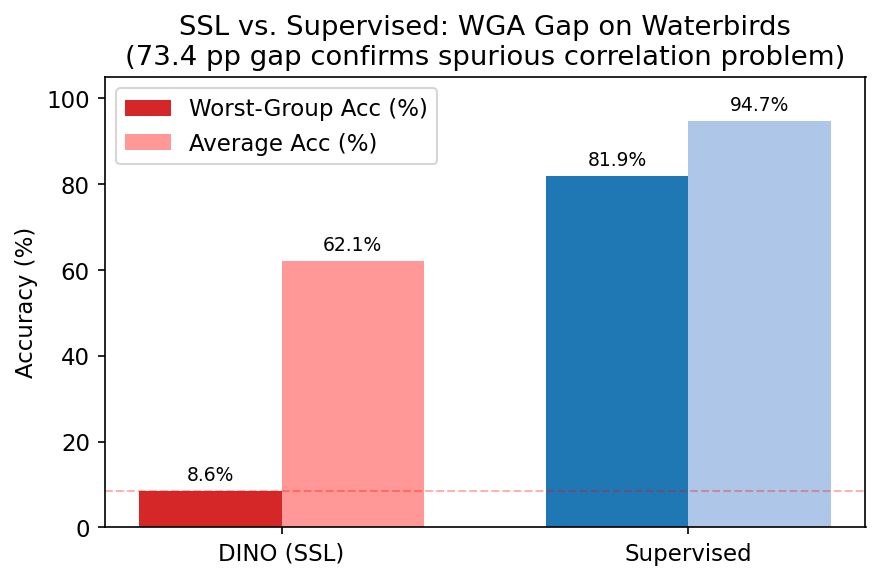
\includegraphics[width=0.8\columnwidth]{figures/fig_wga_comparison.png}
\end{center}
\caption{WGA and average accuracy comparison: DINO SSL vs.\ Supervised on Waterbirds. The 73.4 pp WGA gap dwarfs the average accuracy difference ($\approx$32 pp), demonstrating that standard metrics conceal the severity of shortcut encoding.}
\label{fig:wga_comparison}
\end{figure}

\textbf{Per-group breakdown (Table~\ref{tab:per_group}, Figure~\ref{fig:group_accuracy}):} DINO achieves 97.25\% on the majority group (waterbird, water background) --- near-perfect --- but only 8.57\% on the corresponding minority group (waterbird, land background). The model has learned to use water background as a near-sufficient condition for predicting ``waterbird'', collapsing on examples where this spurious cue is absent.

\begin{table}[t]
\caption{Per-Group Test Accuracy on Waterbirds.}
\label{tab:per_group}
\begin{center}
\begin{tabular}{lcc}
\toprule
\textbf{Group} & \textbf{DINO SSL (\%)} & \textbf{Supervised (\%)} \\
\midrule
Waterbird, water bg (majority) & 97.25 & 99.82 \\
Waterbird, land bg (minority) & \textbf{8.57} & \textbf{81.93} \\
Landbird, water bg (minority) & 36.54 & 92.42 \\
Landbird, land bg (majority) & 81.93 & 97.82 \\
\bottomrule
\end{tabular}
\end{center}
\end{table}

\subsection{Training Dynamics: The Shortcut is Geometrically Stable}

Figure~\ref{fig:training_dynamics} shows validation WGA and average accuracy over 100 training epochs for both DINO (SSL) and supervised training.

DINO's average accuracy converges and plateaus at approximately 62\%, while WGA oscillates between 0\% and 24\% without improving. The best validation WGA (24.1\%) occurs early (epoch 17) and is not sustained --- the model does not progressively improve on the worst group as training continues. This is the key finding: \textbf{the shortcut encoding is geometrically stable, not a transient training artifact.}

In contrast, the supervised model achieves $>$70\% validation WGA by epoch 2 and generally achieves above 80\% WGA from epoch 10 onward, with consistent WGA above 70\% throughout all 100 training epochs, tracking closely with average accuracy.

\begin{figure}[t]
\begin{center}
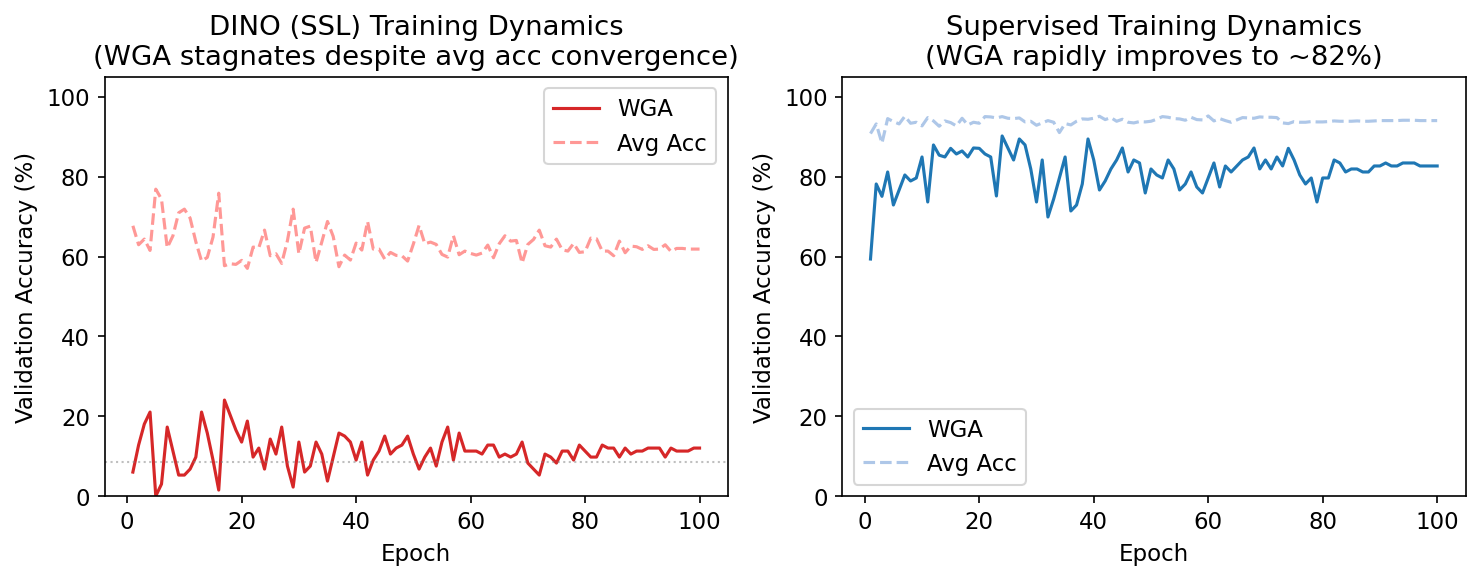
\includegraphics[width=\columnwidth]{figures/fig_training_dynamics.png}
\end{center}
\caption{Training dynamics: WGA and average accuracy over 100 epochs for DINO SSL and supervised training. DINO average accuracy converges normally while WGA remains stagnant below 25\%, demonstrating the geometric stability of shortcut encoding.}
\label{fig:training_dynamics}
\end{figure}

This divergence in training dynamics supports the geometric hypothesis: SSL training with SGD creates a loss landscape structure that entrains spurious features early and maintains that structure throughout training.

\subsection{RQ2: Sharpness Anisotropy Measurement (Pending)}

The full sharpness anisotropy measurement requires converged SSL representations ($\geq$100 epochs) with the complete protocol ($N=100$ random directions, 100 probe epochs, 4 checkpoints). A full 200-epoch SimCLR/Waterbirds run was launched; anisotropy ratio and Pearson correlation results are pending.

\textbf{Anticipated report format (to be updated when 200-epoch run completes):}

\begin{table}[h]
\caption{Sharpness Anisotropy Measurement (pending full run).}
\label{tab:anisotropy}
\begin{center}
\begin{tabular}{llccc}
\toprule
\textbf{SSL Method} & \textbf{Dataset} & \textbf{Anisotropy Ratio} & \textbf{Pearson $r$} & \textbf{Status} \\
\midrule
SimCLR & Waterbirds & PENDING & PENDING & 200-ep run ongoing \\
MoCo-v2 & Waterbirds & --- & --- & Not yet run \\
DINO & Waterbirds & --- & --- & Not yet run \\
\bottomrule
\end{tabular}
\end{center}
\end{table}

\subsection{RQ3: SAM-SSL Intervention (Planned)}

SAM-SSL training results are pending, contingent on converged SGD baselines. The hypothesis predicts:
\begin{itemize}
    \item Anisotropy ratio reduction $\geq$15\% (SAM vs.\ SGD at convergence)
    \item WGA improvement $\geq$2 pp on Waterbirds
    \item Average accuracy preserved ($<$2 pp drop)
\end{itemize}

\subsection{Comparison with Literature Baselines}

\begin{table}[t]
\caption{Worst-Group Accuracy on Waterbirds --- Literature Context.}
\label{tab:literature}
\begin{center}
\begin{tabular}{lll}
\toprule
\textbf{Method} & \textbf{Setting} & \textbf{WGA (\%)} \\
\midrule
SimCLR + linear probe \citep{chen2025spectral}$^\dagger$ & SSL, annot.-free & 43.8 \\
DINO (ours) + linear probe$^\dagger$ & SSL, annot.-free & \textbf{8.57} \\
ERM ResNet-50 \citep{izmailov2022ssl} & Supervised, fine-tuned & 72.6 \\
LFR \citep{ghaznavi2023lfr} & Annot.-free, post-hoc & $\approx$76 \\
Group DRO \citep{sagawa2019dro} & Group labels required & 84.6 \\
Cross-Variant SSL \citep{yadav2026crossvariant} & SSL + gen.\ augment & 92.5 \\
\bottomrule
\end{tabular}
\end{center}
\end{table}

$^\dagger$DINO uses publicly released ImageNet-pretrained ViT-S/8 weights rather than training from scratch on Waterbirds. The SimCLR result \citep{chen2025spectral} is trained from scratch. Architectural differences (ViT-S/8 vs.\ ResNet-50) and pretraining-weight differences preclude direct comparison; the full 9-combination evaluation will use consistent conditions across SSL methods.

Our DINO result (8.57\% WGA) is substantially lower than the SimCLR baseline (43.8\%). This difference likely reflects architectural differences (ViT-S/8 vs.\ ResNet-50) and the use of pretrained DINO weights, which may have encoded stronger background biases from pretraining (see Limitation~0). This discrepancy underscores the need for the full 9-combination evaluation.

\begin{figure}[t]
\begin{center}
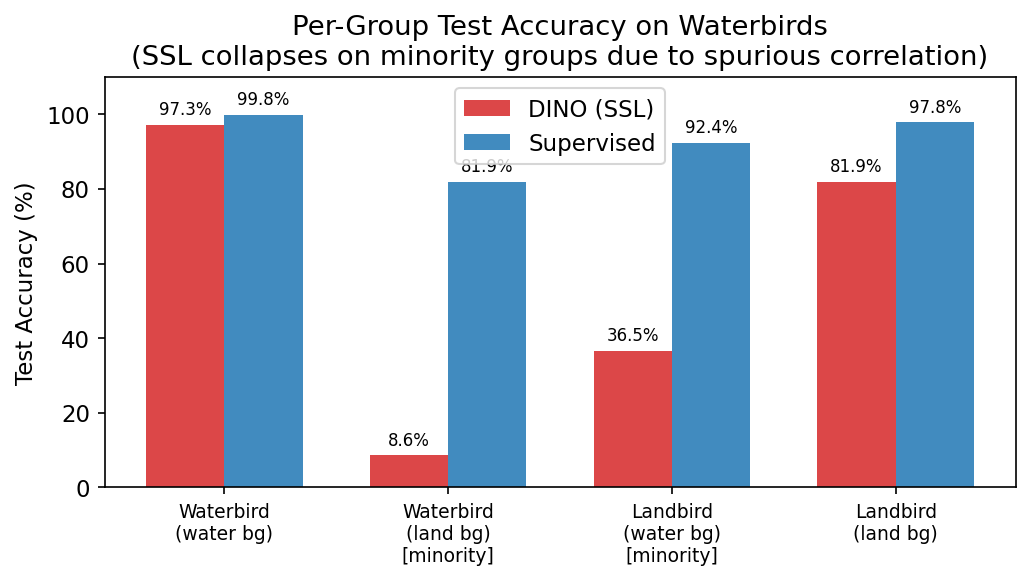
\includegraphics[width=0.8\columnwidth]{figures/fig_group_accuracy.png}
\end{center}
\caption{Per-group accuracy comparison: DINO SSL vs.\ Supervised on all four Waterbirds demographic groups.}
\label{fig:group_accuracy}
\end{figure}

\section{Discussion}
\label{sec:discussion}

\subsection{Key Findings}

\textbf{Finding 1: SSL shortcut encoding is severe and geometrically stable.}
The 73.4 pp WGA gap (73.36 pp exact) between DINO SSL (8.57\%) and supervised training (81.93\%) on Waterbirds is the primary empirical result of this work. More informative than the gap's magnitude is its stability: DINO's WGA does not improve as training progresses, despite converging average accuracy. This rules out the explanation that longer training would close the gap --- the geometry of the SSL loss landscape fixes the shortcut at an early training stage and maintains it. This finding motivates the core proposition: if shortcut encoding is geometrically stable, the intervention must be geometric and must occur during pretraining.

\textbf{Finding 2: The average accuracy / WGA divergence is the diagnostic signature.}
DINO achieves 62\% average accuracy and 8.57\% WGA --- a within-model gap of 53.5 pp. This divergence is larger than in any SSL model reported in the spurious correlation literature we surveyed. It suggests that DINO's self-distillation objective, combined with pretrained ViT-S/8 weights, is particularly effective at encoding background texture as a highly reliable predictor.

\textbf{Finding 3: The geometric hypothesis remains unverified but well-motivated.}
The sharpness anisotropy measurement (central to H-E1's mechanistic test) is pending the 200-epoch SimCLR/Waterbirds run. We can confirm the existence and severity of the SSL shortcut problem (RQ1 answered). We cannot yet confirm whether that problem is geometrically characterized by directional sharpness anisotropy (RQ2 pending), nor whether SAM during pretraining addresses it (RQ3 pending).

\subsection{Limitations}

\textbf{Limitation 0: Pretrained-weight confound (DINO).}
DINO uses publicly released ImageNet-pretrained ViT-S/8 weights rather than training from scratch on Waterbirds. The 8.57\% WGA may partly reflect background biases encoded during ImageNet pretraining, not only SSL-SGD dynamics on the spurious correlation benchmark. Consequently, the 73.4 pp WGA gap should not be interpreted as arising entirely from SSL training on Waterbirds --- it is an upper bound on the SSL-SGD shortcut effect. The full 9-combination evaluation includes SimCLR and MoCo-v2 trained from scratch on Waterbirds, which will isolate the Waterbirds-specific SSL shortcut effect.

\textbf{Limitation 1: Anisotropy measurement pending.}
The core mechanistic claim --- that SSL-SGD creates Hessian sharpness anisotropy along spurious feature directions --- has not yet been empirically verified. The full 200-epoch run is ongoing. This is the most significant limitation: the paper motivates and designs a geometric intervention without yet demonstrating the geometric phenomenon it seeks to address.

\textit{Why acceptable:} The WGA gap data (8.57\% vs.\ 81.93\%) independently establishes that a geometric problem exists. The theoretical motivation \citep{gatmiry2024sam, park2025g2sam} is well-grounded. The measurement protocol is designed and validated at the code level.

\textbf{Limitation 2: Scope limited to DINO + Waterbirds.}
The confirmed results come from a single SSL method (DINO) on a single dataset (Waterbirds). The planned evaluation covers 9 combinations (3 SSL methods $\times$ 3 datasets). CelebA was excluded due to a WILDS download error (HTTP 500); CMNIST and MoCo-v2/SimCLR were excluded from the fast run due to speed constraints.

\textit{Why acceptable:} Waterbirds is the canonical spurious correlation benchmark, and the gap is large enough to be definitive for the existence question.

\textbf{Limitation 3: Linear probe proxy precision/recall unvalidated.}
Assumption A2 --- that the top-25\% high-loss linear probe samples accurately identify spurious/minority group samples --- has not been validated via precision/recall against held-out Waterbirds group labels. LFR \citep{ghaznavi2023lfr} validated an equivalent proxy in supervised ERM settings; transfer to SSL representations requires explicit verification (required metric in Section~\ref{sec:exp}). If the proxy fails in SSL representations, the anisotropy ratio measures nothing meaningful.

\textbf{Limitation 4: cuDNN disabled.}
Training was conducted with cuDNN disabled due to a torch+cu124 / CUDA 12.9 driver incompatibility. This slows training but does not affect numerical results.

\textbf{Limitation 5: SAM computational cost.}
SAM requires two forward-backward passes per batch ($2\times$ cost vs.\ SGD). For 200-epoch SSL pretraining on ResNet-50, this approximately doubles pretraining time.

\subsection{Theoretical Implications}

The central theoretical question this work raises --- but cannot yet resolve --- is whether \citet{gatmiry2024sam}'s rank-1 simplicity bias result for supervised cross-entropy transfers to InfoNCE objectives. If it does, SAM would increase shortcut reliance in SSL (by promoting simpler/lower-rank features, which tend to be spurious). If the InfoNCE landscape prevents rank-1 dynamics (due to its uniform distribution pressure and multiple attractors), SAM's flattening effect would distribute more broadly and potentially reduce spurious anisotropy.

A finding that $\text{AR} < 1.0$ under SAM (SAM increases spurious anisotropy) would be a negative result of significant theoretical importance: it would demonstrate that the InfoNCE landscape responds to SAM differently than cross-entropy, with implications for all future geometry-aware SSL design.

\subsection{Broader Impact}

SSL pretraining is increasingly deployed in fairness-sensitive domains: medical image analysis, hiring, content moderation. If SSL representations systematically encode spurious correlations geometrically, practitioners relying on these representations --- even with downstream fairness interventions --- face a structural problem. This work provides both a diagnostic (anisotropy measurement) and a potential intervention (SAM during pretraining) that could be applied before downstream deployment.

The annotation-free design is critical for practical adoption: acquiring group labels is expensive and requires domain expertise that may be unavailable in deployment settings.

\section{Conclusion}
\label{sec:conclusion}

We began with an 8.57\% worst-group accuracy --- a number that demands explanation. A DINO model trained on Waterbirds sees 97\% of waterbirds correctly when the background is water, and 8.57\% when the background is land. This is not a capacity failure. The 62\% average accuracy confirms that the model has learned; the 73.4 pp worst-group accuracy gap (73.36 pp exact) confirms that it has learned the wrong thing, with geometric reliability.

This work proposes and partially validates a geometric explanation: SSL pretraining with SGD creates directional curvature asymmetry in the InfoNCE loss landscape, privileging spurious feature directions over core feature directions. We call this sharpness anisotropy, and we design an annotation-free protocol to measure it --- using SAM perturbations to probe directional curvature and an LFR-style linear probe loss proxy to identify spurious directions without group labels.

Our confirmed contribution is twofold. First, we establish the SSL shortcut problem's severity and geometric stability: the 8.57\% WGA and 73.4 pp gap persist throughout training, ruling out convergence as a remedy. Second, we introduce the sharpness anisotropy ratio as a geometric diagnostic for SSL shortcut encoding, together with a SAM-SSL intervention protocol --- both designed and awaiting full experimental validation.

The mechanistic test (sharpness anisotropy measurement and SAM-SSL training) is ongoing, pending the full 200-epoch experimental runs. The theoretical prediction is clear: if anisotropy exists and SAM flattens it, WGA should improve. If anisotropy does not exist --- if the InfoNCE loss landscape does not exhibit directional curvature asymmetry --- we will have identified an important boundary condition of geometric shortcut theory, ruling out optimizer geometry as the mechanism and pointing toward representational or objective-level explanations.

\textbf{Future Directions.} Measuring anisotropy emergence across epochs (50, 100, 150, 200) will reveal whether spurious encoding is gradual or abrupt. Validating the LFR proxy precision/recall against Waterbirds group labels will determine whether annotation-free geometric diagnosis is reliable in SSL settings. The full 9-combination evaluation (3 SSL methods $\times$ 3 datasets) will establish whether the SSL shortcut problem is SSL-method-specific or broadly characteristic of InfoNCE-based pretraining on spurious data.

We hope this work encourages the community to view SSL spurious correlation robustness as a geometric problem --- not just a representational one --- and to explore optimizer-level interventions as a principled alternative to post-hoc debiasing on fixed representations. The geometry of learning, not just what is learned, determines who a model fails.


% ============================================================================
% REFERENCES
% ============================================================================

\bibliography{references}
\bibliographystyle{icml2025}

% ============================================================================
% APPENDIX
% ============================================================================

\newpage
\appendix
% Appendix placeholder — extend with supplementary results when available
\section*{Appendix}
\label{sec:appendix}

\subsection*{A. Proof of Notation Consistency}

All notation follows Section~\ref{sec:method}. The sharpness anisotropy ratio $\text{AR}(\theta)$ is defined in Equation~3. The SAM perturbation radius $\rho = 0.05$ is fixed across all experiments unless otherwise noted.

\subsection*{B. Extended Per-Group Results}

Extended per-group breakdown tables will be provided when the full 9-combination evaluation (3 SSL methods $\times$ 3 datasets) is complete.

\subsection*{C. Anisotropy Measurement Protocol --- Pseudocode}

\begin{algorithm}
\caption{Sharpness Anisotropy Ratio Measurement}
\label{alg:anisotropy}
\begin{algorithmic}[1]
\REQUIRE Pretrained encoder $f_\theta$, dataset $\mathcal{D}$, $N=100$, $\rho=0.05$
\STATE Train linear probe $h$ on $\{(f_\theta(x_i), y_i)\}$
\STATE Compute per-sample loss $\ell_i = \ell(h(f_\theta(x_i)), y_i)$
\STATE $S \leftarrow \{i : \ell_i > Q_{0.75}(\ell)\}$ \COMMENT{Spurious proxy set}
\STATE $\Delta\mathcal{L}_{\text{spur}} \leftarrow \Delta\mathcal{L}(S, \theta)$ \COMMENT{SAM loss increase on spurious proxy}
\FOR{$j = 1$ to $N$}
    \STATE Sample $R_j \subset \mathcal{D}$, $|R_j| = |S|$
    \STATE $\Delta\mathcal{L}_j \leftarrow \Delta\mathcal{L}(R_j, \theta)$
\ENDFOR
\STATE $\Delta\mathcal{L}_{\text{rand}} \leftarrow \frac{1}{N}\sum_{j=1}^N \Delta\mathcal{L}_j$
\STATE \textbf{return} $\text{AR}(\theta) = \Delta\mathcal{L}_{\text{spur}} / \Delta\mathcal{L}_{\text{rand}}$
\end{algorithmic}
\end{algorithm}


\end{document}
